\section{Clustering}
Clustering belongs to Unsupervised Learning with the Subcategory Clustering.

\subsection{In General}
Data often has structure. 
But the structure can be hidden by noise.
The goal is to identify hidden patterns among the data.\\
\textbf{Applications:}
\begin{itemize}
  \item Social network analysis
  \item Astronomical data
  \item market segmentation
  \item recommendation systems
\end{itemize}
Same concept as KNN, but taken further.
We try to identify and group data points whose features are similar (close together).
We partition the data into so called ``clusters''.

\subsection{Naive K-means}
\begin{enumerate}
  \item Let us assume we know the number of clusters $k_c$
  \item Initialize the value of $k$ cluster centres ($C_1,C_2,\dots C_{k_c}$)
  \item Assignment:
  \begin{enumerate}
    \item Find the squared Euclidean distance between the centres and all the data points.
    \item Assign each data point to the cluster of the nearest centre.
  \end{enumerate}
  \item Update: Each cluster now potentially has a new centre (mean). Update the centre for each cluster
  \begin{enumerate}
    \item New Centres ($C'_1,C'_2,\dots C'_{k_c}$) = Average of all the data points in the cluster ($1,2, \dots K_c$)
  \end{enumerate}
  \item If some stopping criterion met, Done
  \item Else, go to Assignment step 3
\end{enumerate}

\subsubsection{Calculating cluster center}
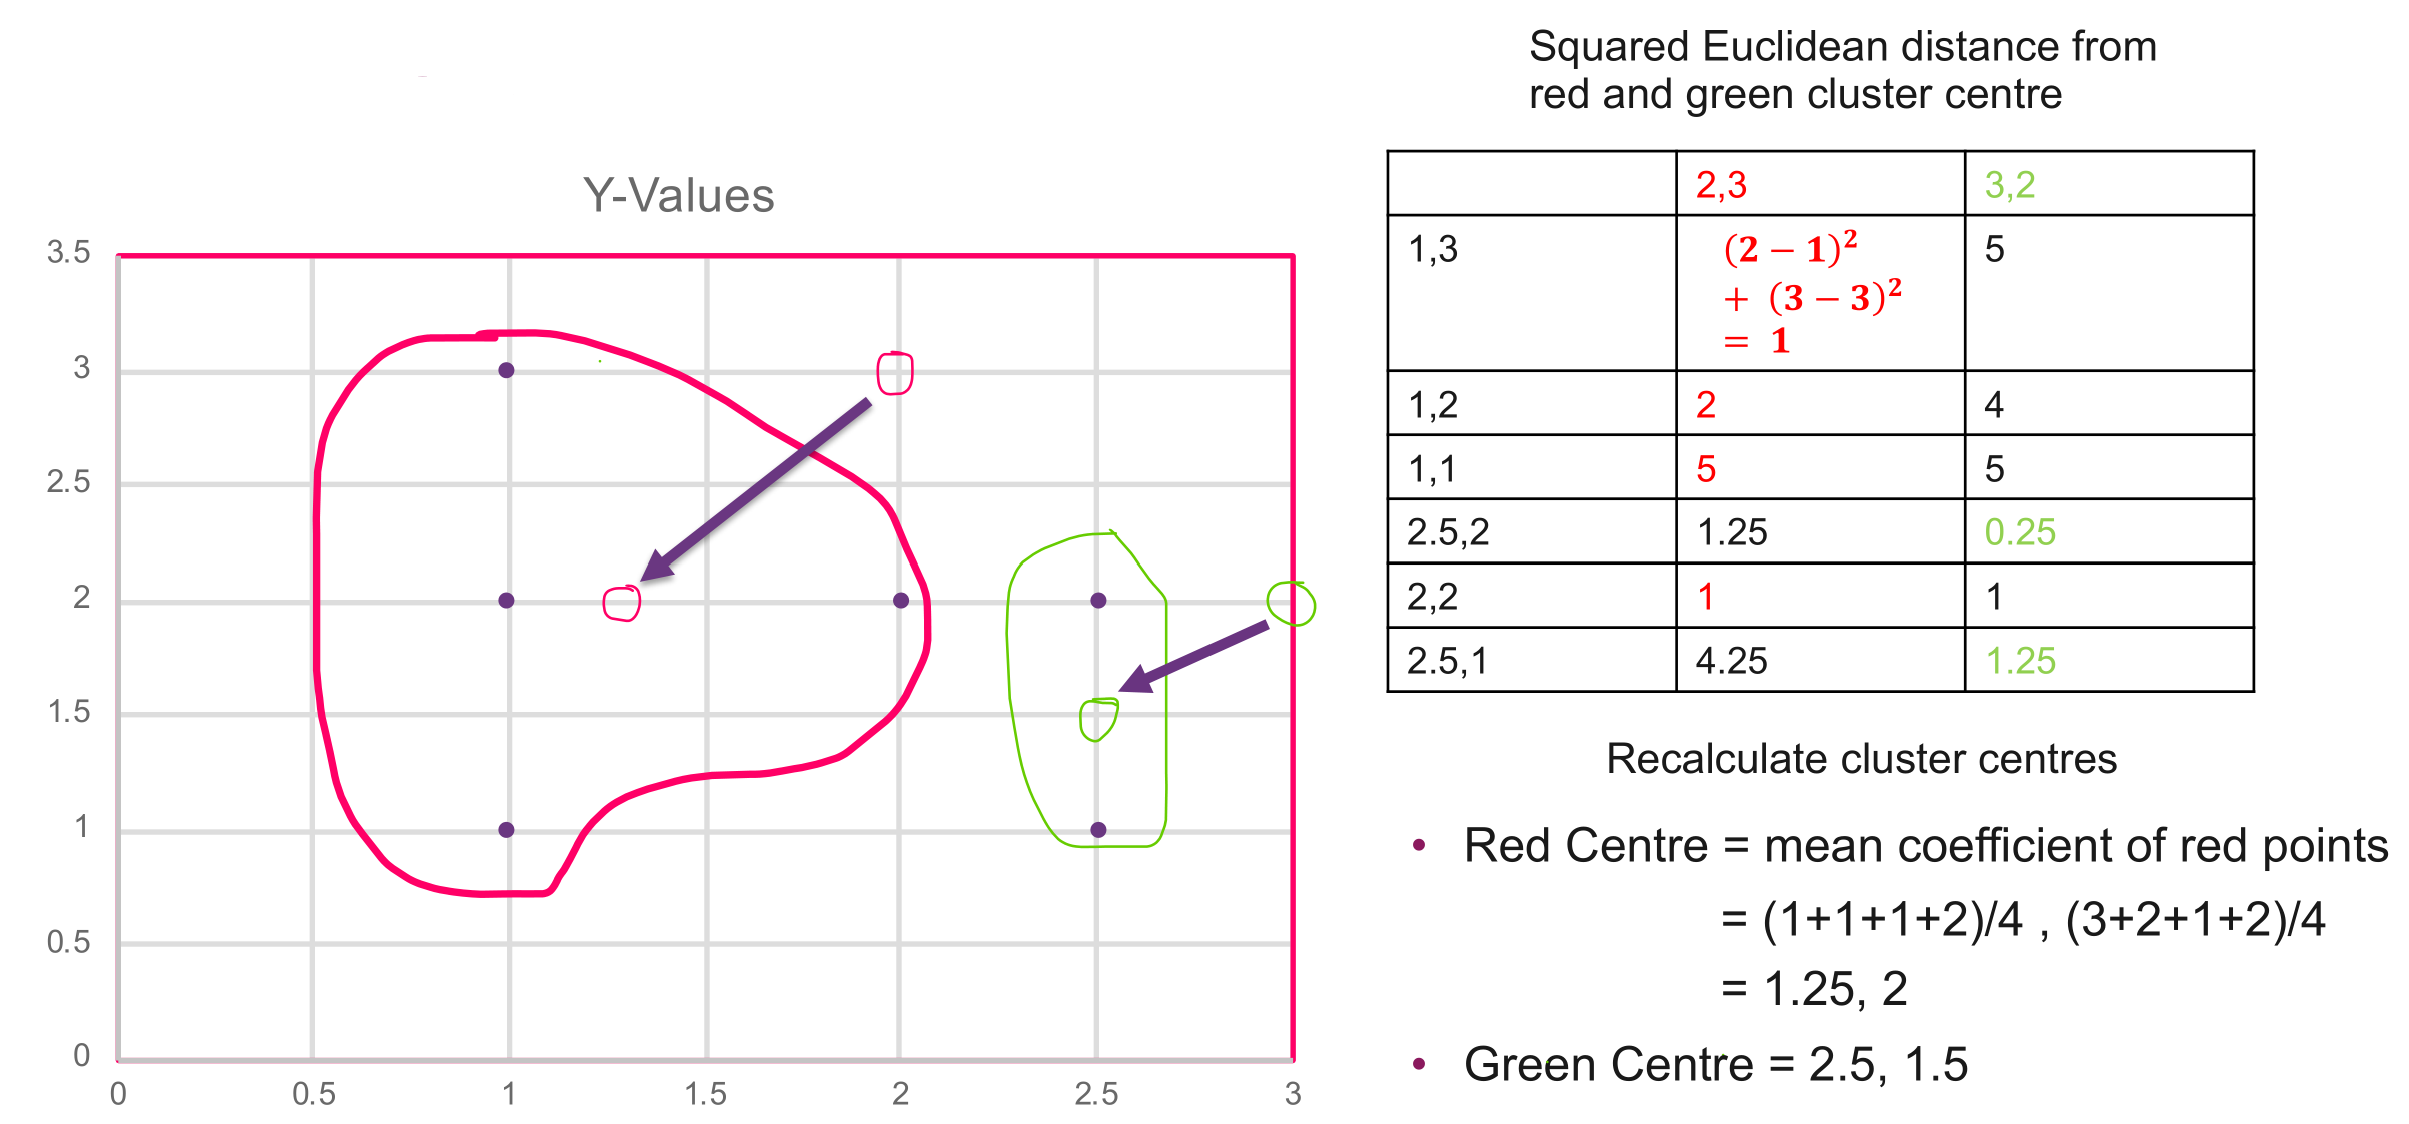
\includegraphics[width=\linewidth]{cluster-center-1.png}\\
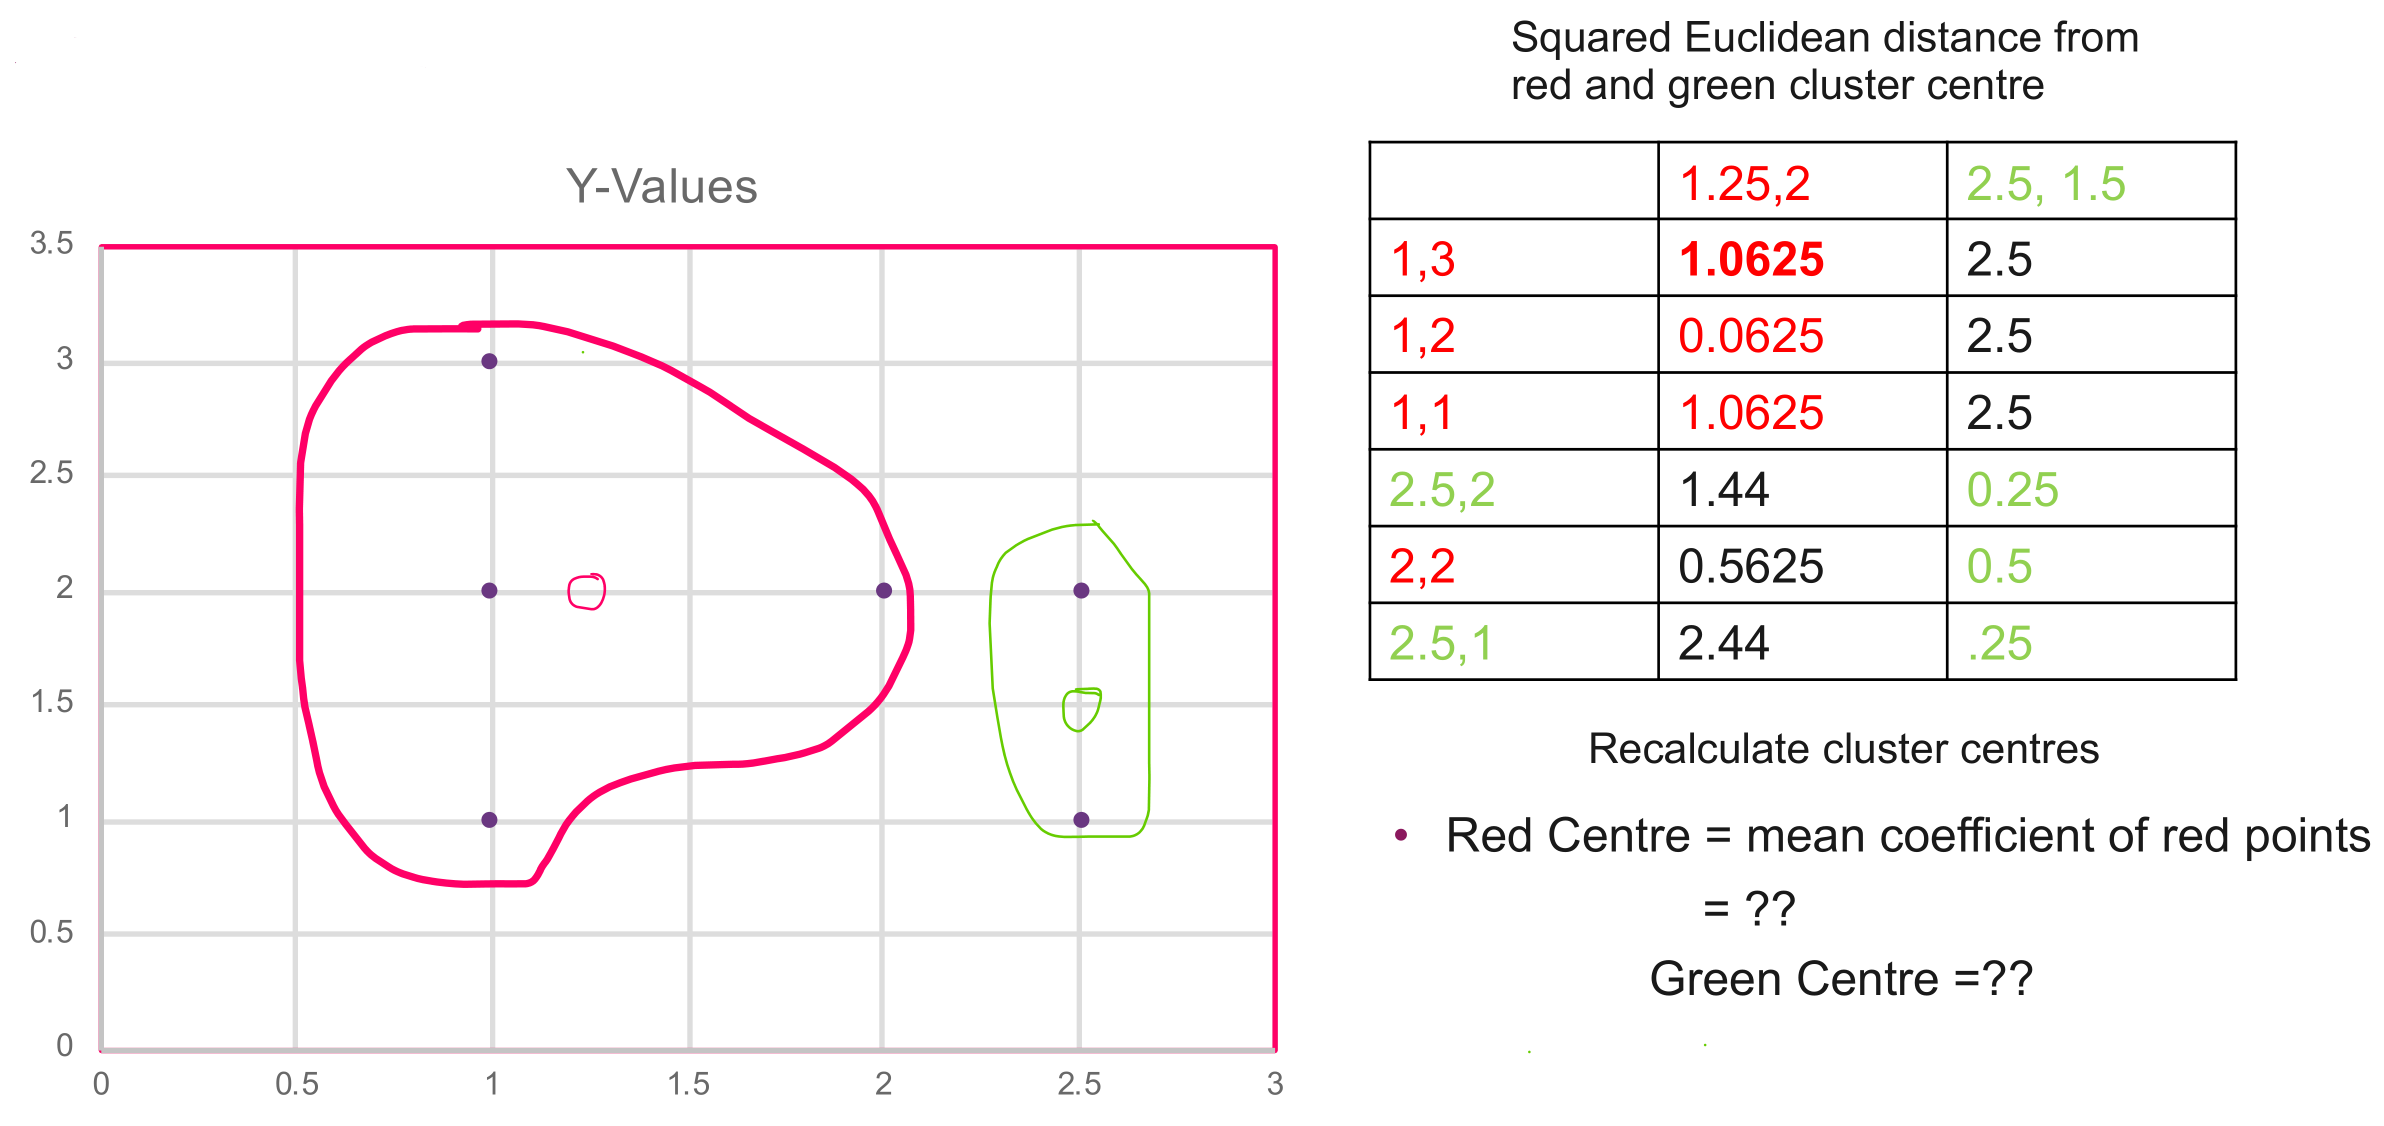
\includegraphics[width=\linewidth]{cluster-center-2.png}

\subsubsection{Stopping Criterion}
\begin{itemize}
    \item When centres don't change (time consuming)
    \item The datapoints assigned to specific cluster remains the same (takes too much time)
    \item The distance of datapoints from their centres $>=$ treshold we have set
    \item Fixed number of iterations have reached (choose wisely)
\end{itemize}

\subsubsection{Initialization}
\begin{itemize}
    \item Performance depends on the random initialization
    \item Some seeds can result in a poor convergence rate
    \item Some seeds can converge to suboptimal clustering
    \item If centres are very close, it takes a lot of iterations to converge
    \item Initialize randomly, run multiple times
\end{itemize}

\subsubsection{Standardization of data}
\begin{itemize}
    \item Features with large values may dominate the distance value
    \item Features over small values will have no impact
    \item Normalize values!
\end{itemize}

\subsubsection{Sklean k-means}
\textbf{Initialization}
\begin{itemize}
    \item Init = K-means++
    \item Only initialization of the centroids will change
    \item Chosen centroids should be far from each other
\end{itemize}
\textbf{max\_iter:}
\begin{itemize}
    \item Number of iterations before stopping
\end{itemize}
\textbf{n\_init:}
\begin{itemize}
    \item Number of time the k-means algorithm will be run with different centroid seeds
\end{itemize}

\subsubsection{Evaluating Cluster Quality}
\begin{itemize}
    \item Make clusters so that for each cluster the distance of each cluster member from its center is minimizes
\end{itemize}
\textbf{Inertia or within-cluster sum-of-squares (WCSS)}
\begin{itemize}
    \item Sum of squared distances to center
    \item As small as possible
\end{itemize}
\subsubsection{WCSS}
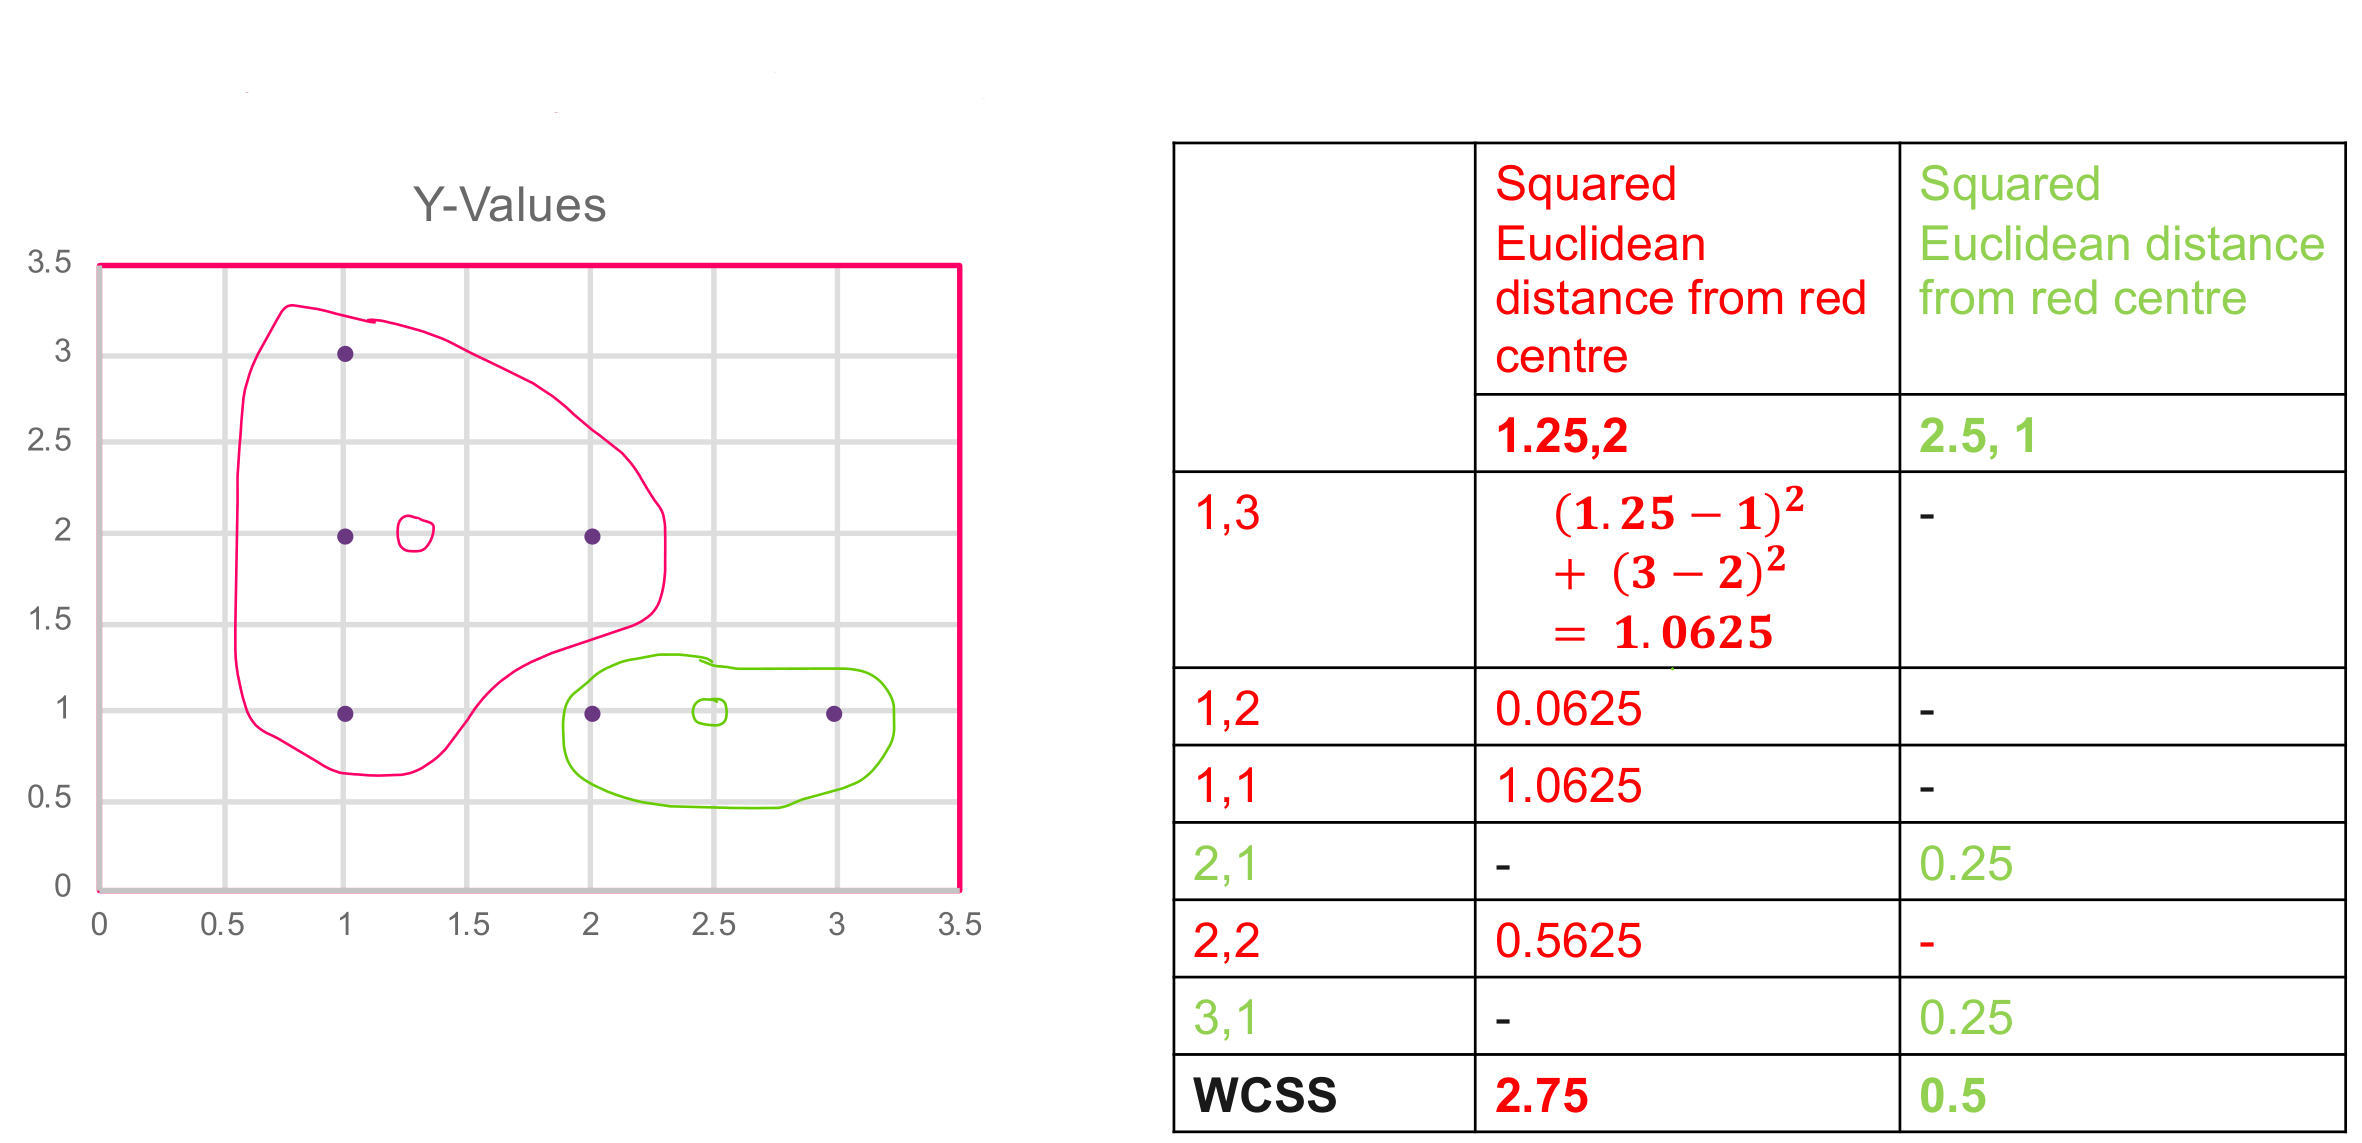
\includegraphics[width=\linewidth]{wcss.png}

\subsubsection{Silhouette Score}
\begin{itemize}
    \item How far the datapoints in one cluster are from the datapoints in another cluster
    \item SS of a point: $\frac{b-a}{max(a,b)}$
    \item a: average intra-cluster distance (distance between each point within)
    \item b: average inter-cluster distance (distance between a cluster and its nearest neighbour)
\end{itemize}
Calculate distance with Pythoagoras:\\
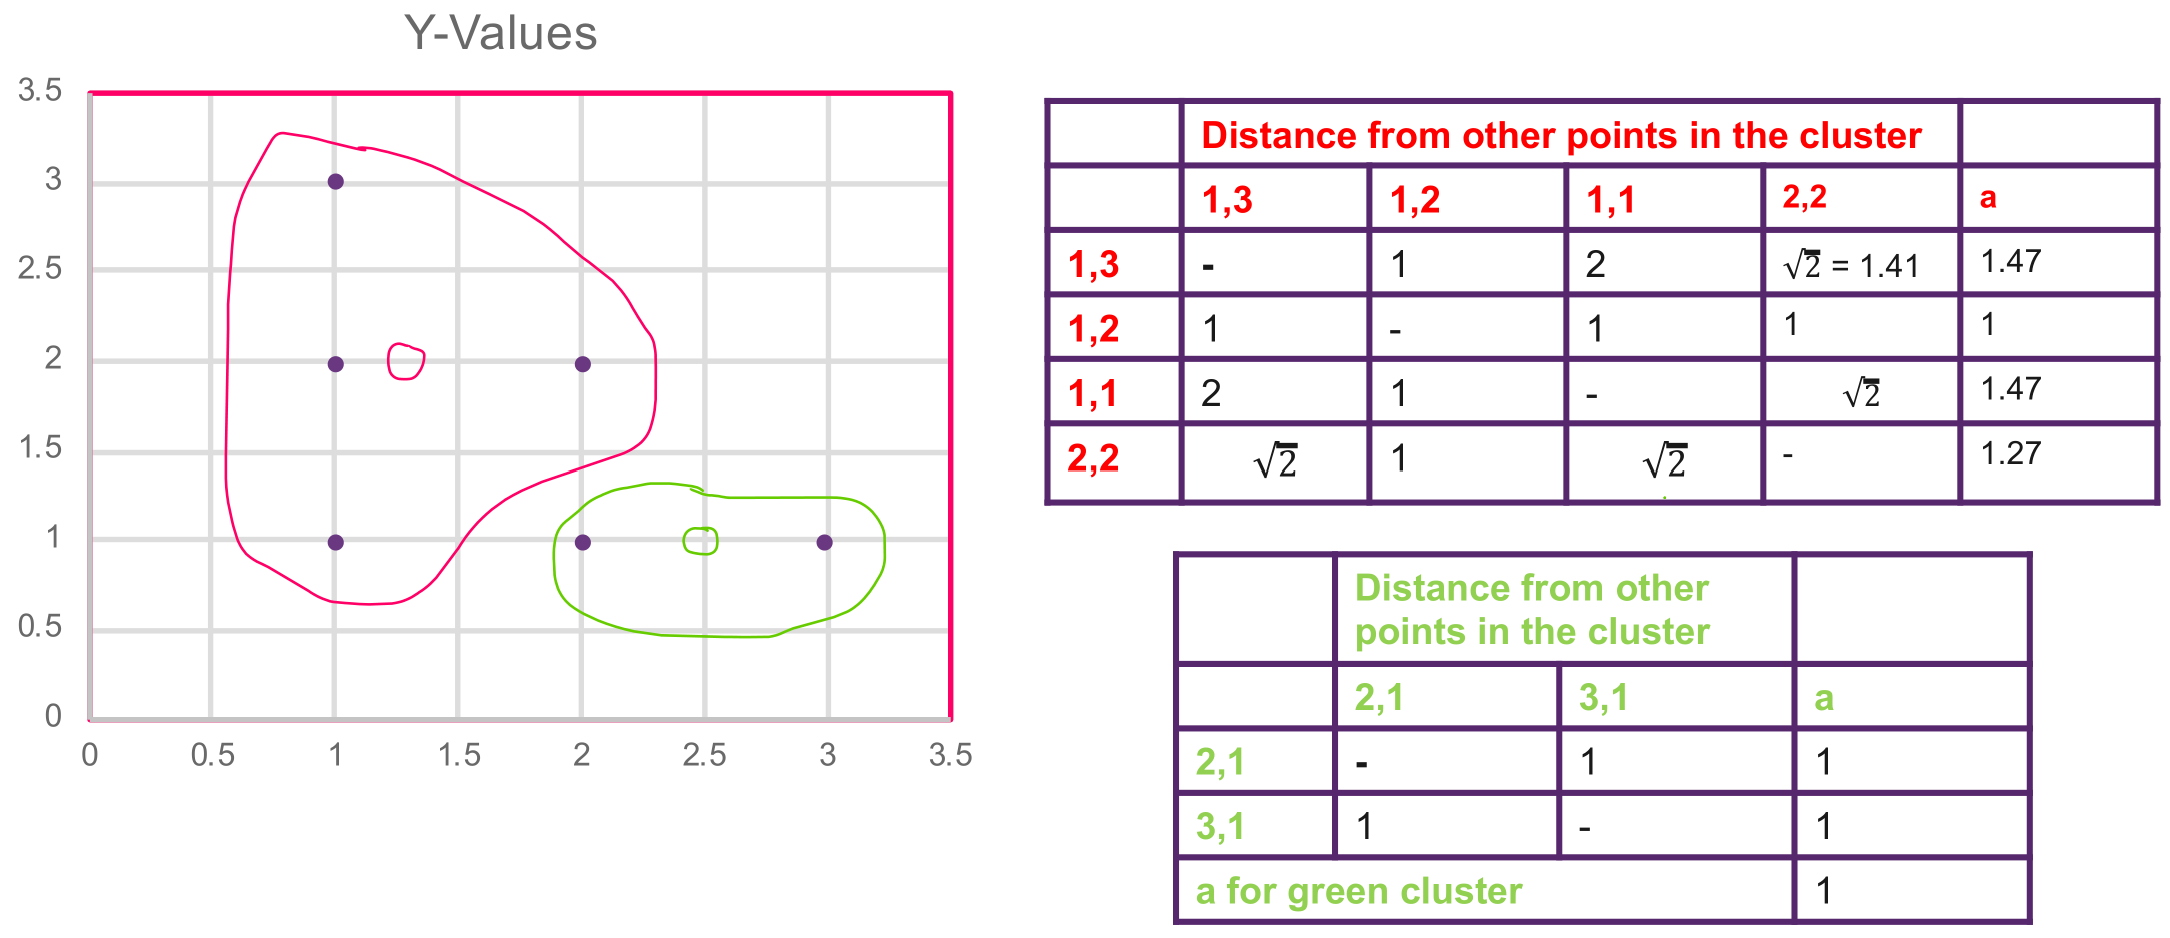
\includegraphics[width=\linewidth]{silhouette-score-1.png}\\
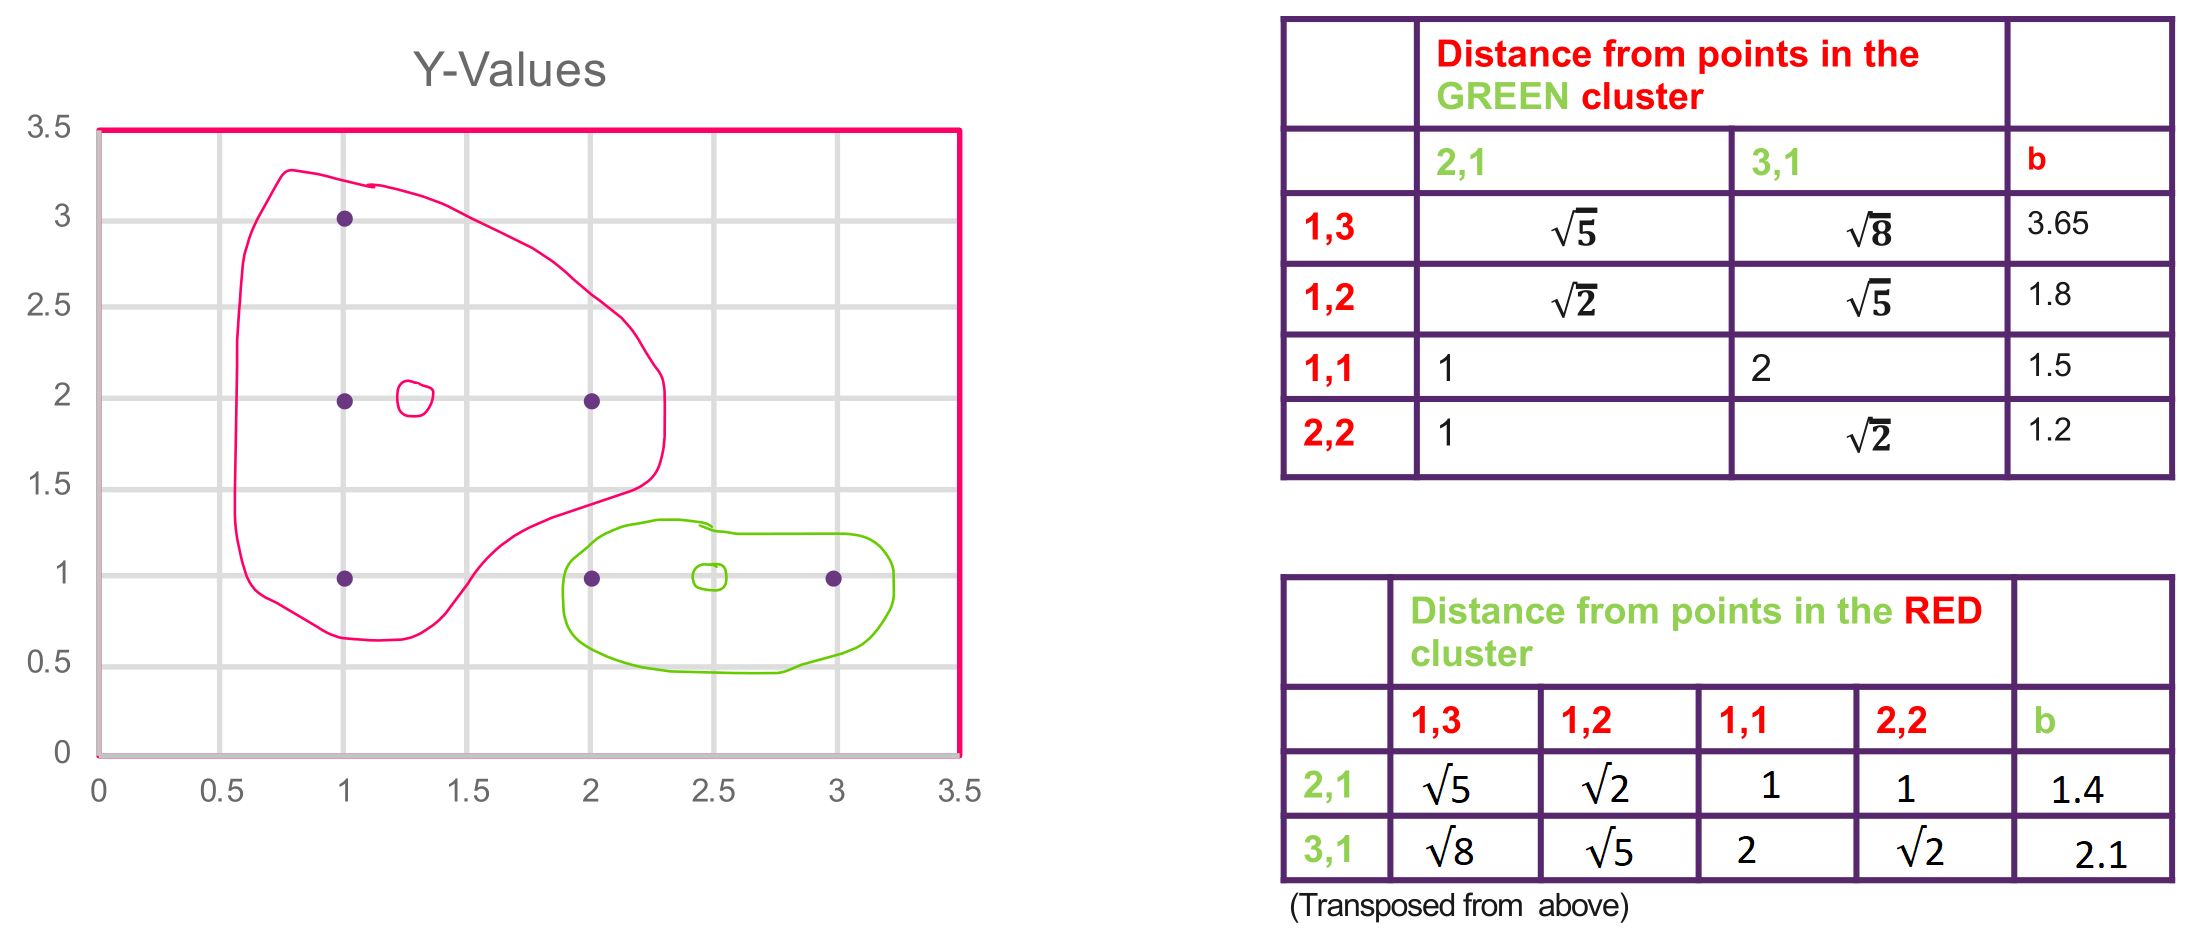
\includegraphics[width=\linewidth]{silhouette-score-2.png}